\chapter{Results}


\section{G3BP1 tethering affects mRNA localization}

Proteins of the G3BP RNA-binding family are key components of SGs.
In mammals, G3BP1 (and its paralog G3BP2) were reported to be essential in nucleating the formation of SGs \cite{kedersha_g3bp-caprin1-usp10_2016}.
SGs can not only be induced by stress (e.g. sodium arsenite) but also by the overexpression of G3BPs \cite{tourriere_rasgap-associated_2003}.
In addition, a recent proteomics-based study by Markmiller et al. \cite{markmiller_context-dependent_2018} showed that "many well-characterized SG proteins (e.g., G3BP1, TIA1, CAPRIN1, PABPC1, FMR1, and ATXN2) were identified as highly significant interactors" suggesting an interplay of SG proteins even in unstressed conditions.
This finding might suggest the formation of an mRNP complex containing SG proteins allowing for a rapid assembly of SGs.

The exact role of G3BPs in SG assembly as well as in unstressed cells is still largely unknown.
As reviewed in Alam and Kenedy \cite{alam_rasputin_2019} various functions have been attributed to this protein family.
These range from transcript destabilization and repression to the polar opposite in transcript stabilization.
Furthermore, G3BP's also showed effects on transcript localization and sequestration to virus-induced foci (reviewed in \cite{zhang_chronic_2019}).
The only consensus is G3BP's involvement in mRNA translational control.
The subsequent experiments attempt to clarify this disunity by analyzing G3BP1's effect on mRNA transcripts at a single-molecule level.
For this reason, I designed an assay to directly tether G3BP1 to reporter mRNAs and thereby allow its effect on translation and mRNA degradation to be measured as well as to promote mRNA accumulation into SGs.

\begin{figure}[b!]
    \centering
    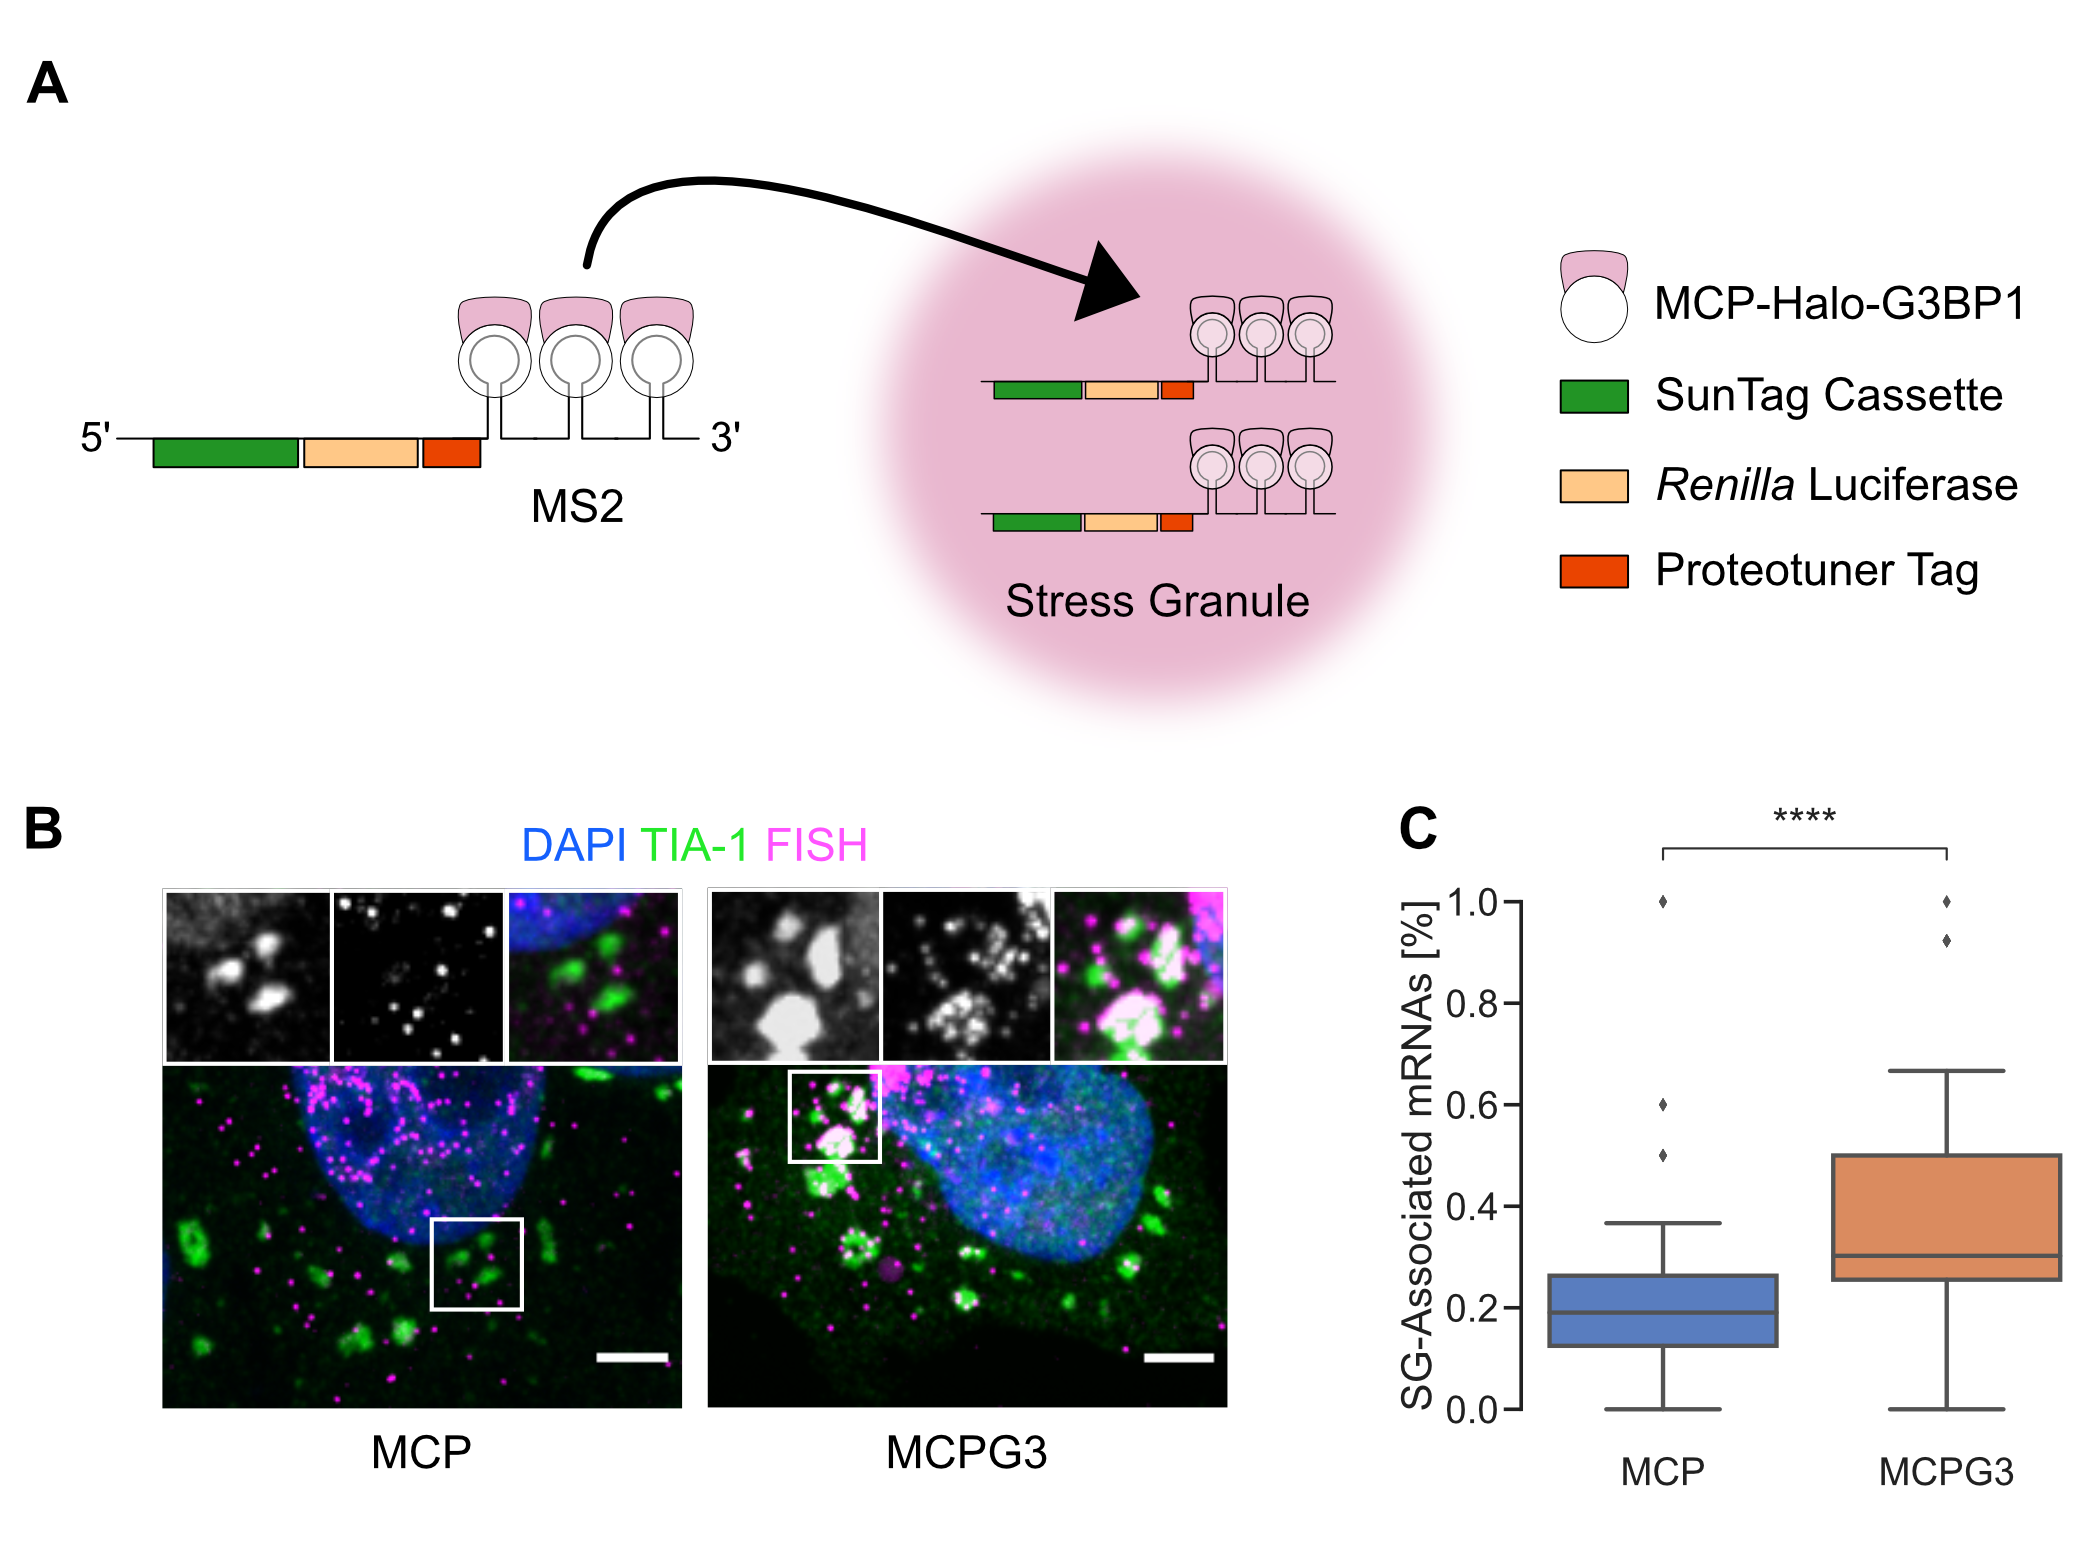
\includegraphics[width=\linewidth]{images/figure2}
    \caption{\textbf{Design of MCPG3.}
        (A) Schematic depiction of MCPG3 function.
        (B) Representative fluorescence images of the SG marker
            TIA-1 and the tethered RNAs.
            To induce SGs, cells were treated with sodium arsenite (1 mM/ml) for 1 hour.
            Pannels show TIA-1, FISH, Merge respectively.
            Scale bars, 10 \textmu m.
        (C) Quantification of the mRNA recruitment to SGs.
            Number of cells quantified (left to right): 27, 21. Two replicates.
    }
    \label{fig:mcp_images}
\end{figure}

This study focussed on a reporter RNA containing a SunTag cassette, the gene encoding for \textit{Renilla} luciferase, a proteotuner tag, and MS2 stem-loops (Figure \ref{fig:mcp_images}A).
In order to promote mRNA recruitment to SGs, I fused G3BP1 MCP-Halo (abbreviated as MCPG3).
The construct was validated by FISH against the reporter RNA followed by immunofluorescence for the endogenous SG marker TIA-1 \cite{kedersha_rna-binding_1999} (Figure \ref{fig:mcp_images}B).
SGs were induced by sodium arsenite treatment (1 mM/ml for 1 hour).
As a control, an identical construct only lacking G3BP1 fusion was used.
Both by visual inspection as well as by mRNA quantification (Figure \ref{fig:mcp_images}C), a significant difference in SG association can be seen.
MCPG3 shows an approximately two-fold increase in SG associated mRNAs compared to the control while not causing mRNA aggregation in unstressed conditions (Supplementary Figure \ref{fig:mcp_supplement}).
Taken together, fusing G3BP1 to MCP seems to be a reliable way to recruit functional G3BP1 to the local vicinity of mRNAs and thereby promote localization to SGs.


\subsection{Reporter expression is impacted by G3BP1} \label{mcp_luciferase}

Having shown that G3BP1 can be recruited to mRNAs, I wanted to investigate the effect on translational activity. \textit{Renilla} luciferase assays are used to measure reporter expression on a global level.
As G3BP1 was shown to be involved in stress-induced events as well as in unstressed conditions, the luciferase activity at multiple time points in unstressed cells as well as in cells recovering from oxidative stress was measured.

\begin{figure}[t!]
    \centering
    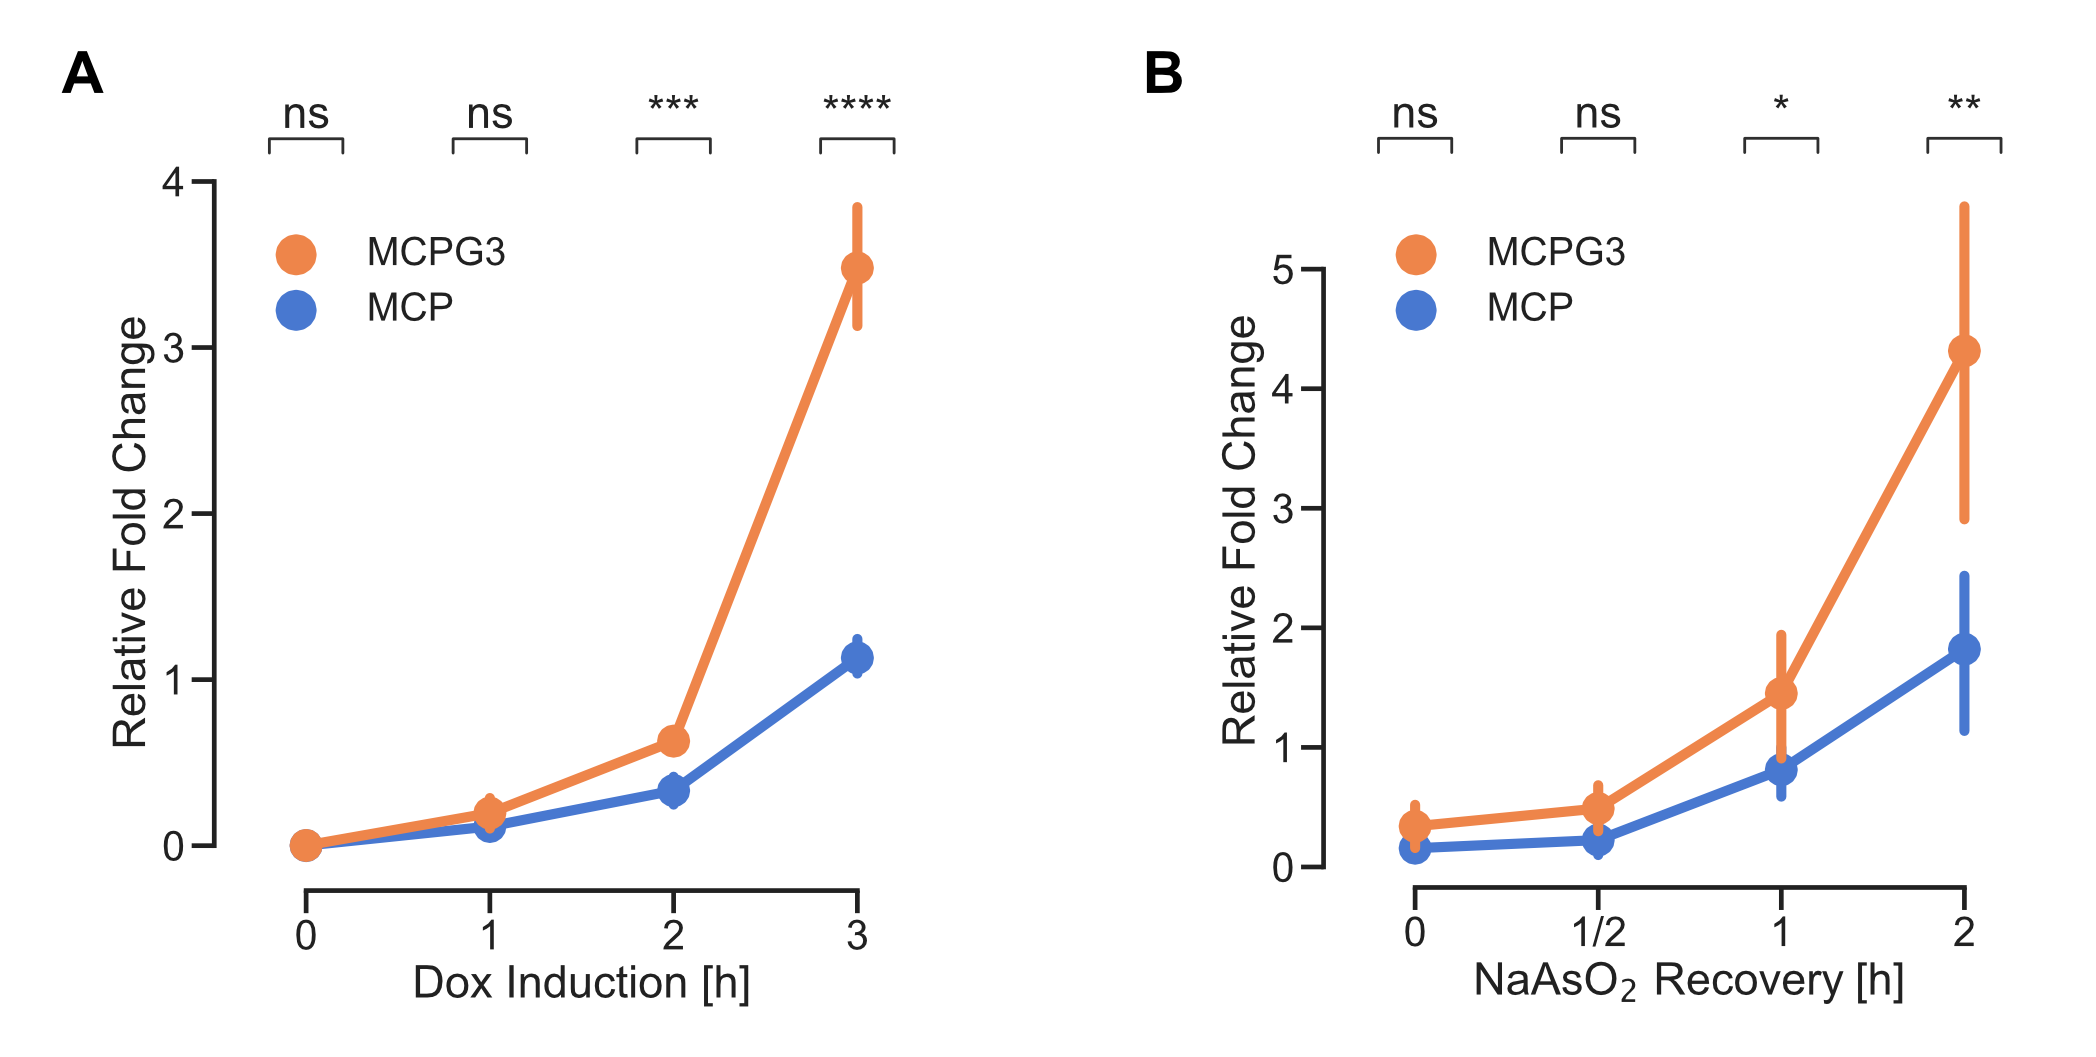
\includegraphics[width=\linewidth]{images/figure3}
    \caption{\textbf{G3BP1 tethering increases reporter translational activity.}
        (A) Luciferase assays at different time points during induction.
        (B) Sodium arsenite stress recovery time points after induction.
            Cells were induced for 3 hours and stressed with sodium arsenite (1 mM/ml) in the last hour.
            Timepoint capture started immediately after washing out stressor.
        (A and B) Data normalized to the 3-hour induction condition of MCP. Five replicates.   
    }
    \label{fig:mcp_luciferase}
\end{figure}

In unstressed cells, G3BP1 recruitment resulted in increased luciferase readings over time (Figure \ref{fig:mcp_luciferase}A).
This suggests that the presence of G3BP1 on a transcript might promote protein synthesis.
Comparing both constructs during stress recovery, one can observe a slightly less significant but still noticeable increase in luciferase activity for MCPG3 expressing cells (Figure \ref{fig:mcp_luciferase}B).
Interestingly, the largest effects are at later time points and during non-stress conditions while not being immediately after stress recovery.
Undisclosed preliminary experiments using different durations of stress have yielded similar results.
SGs have been observed to persist between a few minutes to hours after removal of the stressor \cite{chen_relationships_2017}.
This correlates with the time when an increase in luciferase activity can be observed again.


\subsection{G3BP1 does not alter mRNA translation}\label{mcp_suntag}

The observed differences in luciferase activity described in Section \ref{mcp_luciferase} can result from various causes.
These differences in reporter protein synthesis levels could arise from an increase in translational activity of mRNAs or an increase in mRNA stability.
To investigate the former possibility, I decided to use SunTag imaging, to directly quantify translational activity (see Section \ref{translation_site_imaging}).

In SunTag imaging, the fluorescence intensity is a direct measure of translation rate.
Therefore, to analyze the translation activity of MCPG3-bound mRNAs, the intensity of translation site spots was quantified over at least four consecutive timeframes with a maximum of one gap frame.

When comparing SunTag tracks in unstressed cells expressing MCPG3 or control MCP (Figure \ref{fig:mcp_suntag}A), both conditions show similar fluorescence intensities suggesting G3BP1 does not have a major effect on mRNA translation rates.
Similarly, the grouping of SunTag tracks into segmented cells shows comparable mean intensities in cells expressing MCPG3 or control MCP.
Equivalently to the image-level analysis, cellular intensities (Figure \ref{fig:mcp_suntag}B) do not yield different results.
The average intensity of all tracks per cell does not appear to be affected by G3BP1 fusion.

During stress conditions, most mRNAs get translationally silenced (reviewed in Holcik and Sonenberg \cite{holcik_translational_2005}).
To image translation sites despite this silencing, images were acquired 15 to 30 minutes after removing the stressor.
Nonetheless, cells did not fully recover the translational silencing leading to lower readings of fluorescent intensity in the stress condition compared to unstressed cells.
However, in this case, as well, G3BP1 tethering does not lead to significant differences in translational activity.

Lastly, translation can also increase due to a higher number of translating transcripts per cell.
However, as is evident from Figure \ref{fig:mcp_suntag}C the number of translating tracks stays consistent in all experiments.
This suggests that G3BP1 does not have a profound impact on translation activity.

\vspace*{\fill}
\begin{figure}[b!]
    \centering
    \caption{\textbf{G3BP1 does not affect translational activity.}
        (A) Distribution of the mean fluorescence intensity of tracked
            mRNAs in the full-sized image (without cellular segmentation).
        (B) Track intensity averaged per cell.
        (A and B) Data normalized to the Dox induction condition for MCP.
            The total number of tracks (left to right): 715, 1064, 997, 3442.
        (C) The number of tracks registered per cell.
        (B and C) The total number of cells (left to right): 48, 77, 31, 48. Single replicate.
    }
    \end{figure}
    \addtocounter{figure}{-1}
    \begin{figure} [H]
    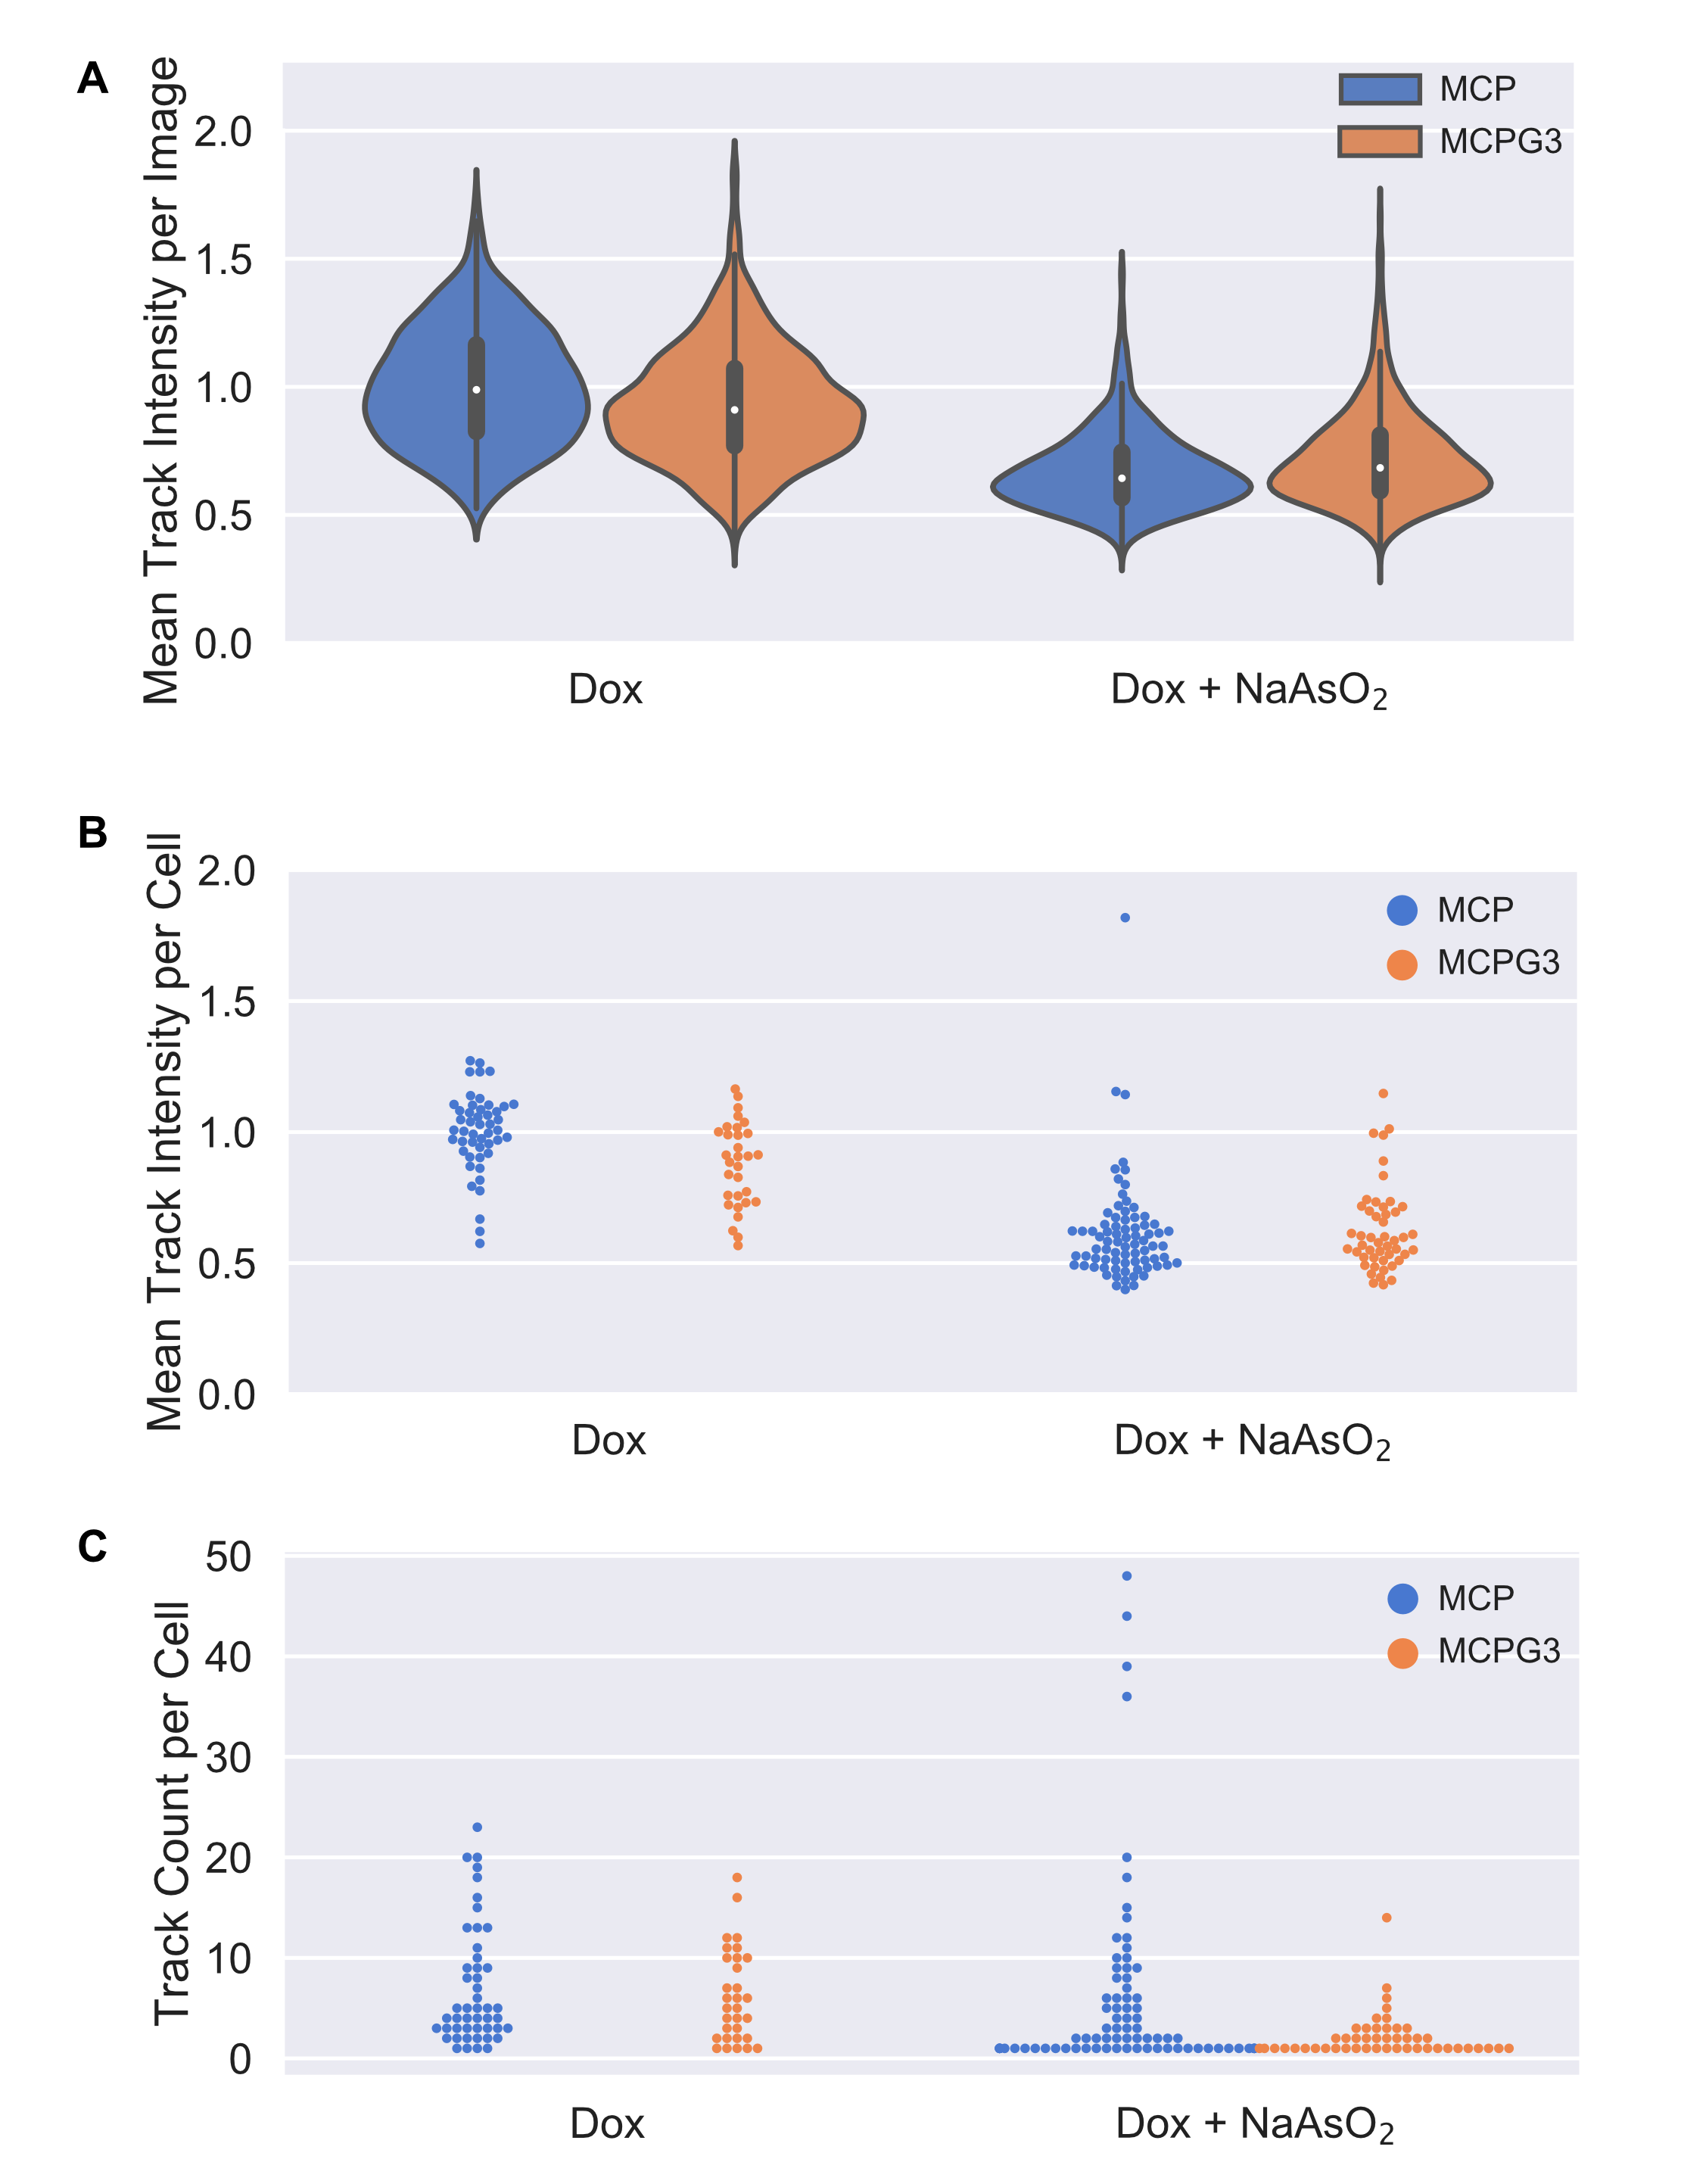
\includegraphics[width=\linewidth]{images/figure4}
    \caption{(On the previous page.)}
    \label{fig:mcp_suntag}
\end{figure}


\subsection{Transcript stability is affected by G3BP1 tethering} \label{mcp_treat}

SunTag measurements (see Section \ref{mcp_suntag}) did not suggest any effect of G3BP1 on translational activity.
Alternatively, a decrease in mRNA degradation could also explain the increased \textit{Renilla} luciferase readings.
To ask whether G3BP1 has an mRNA stabilizing effect, I compared the half-lives of transcripts between MCPG3 and the control using 3(three)$'$-RNA end accumulation during turnover (TREAT) \cite{horvathova_dynamics_2017}.

TREAT uses a slightly modified reporter mRNA containing viral RNA pseudo-knot (PK) structures upstream of the MS2 stem-loops.
These PKs can block Xrn1 mediated 5$'$-3$'$ degradation of a transcript by sequestering the 5$'$ phosphate group \cite{kieft_new_2015}.
Subsequently, by using FISH probes against \textit{Renilla} luciferase upstream of PKs (showing intact mRNAs) and FISH probes against MS2 stem-loops downstream of PKs (showing both intact and degraded mRNAs) one can quantify the number of degradation intermediates.

To look at transcript stabilization, a cell line expressing the aforementioned TREAT mRNA reporter was used.
Five time points were chosen to match TREAT half-life after a 1 hour induction followed by thorough washing to remove doxycycline to halt any further transcription.
As can be seen in Figure \ref{fig:mcp_treat}A, transcripts are exported from the nucleus into the cytosol over the course of the experiment.
This suggests that no new transcripts are produced in the nucleus and that MCPG3 does not negatively affect nuclear export.

When comparing the percentage of intact mRNAs, i.e. transcripts still containing FISH spots against both \textit{Renilla} luciferase and MS2, between MCPG3 and the control, I observed a significant difference (Figure \ref{fig:mcp_treat}B).
The G3BP1 fusion shows a significant reduction in degraded transcripts compared to the control suggesting an increase in mRNA stability.
This effect is not reflected in the translation site-based mRNA count from the SunTag measurements (see Section \ref{mcp_suntag}) which might arise from the nature of the SunTag cassette that will be discussed in the following Section \ref{spaghetti}.


\begin{figure}[h]
    \centering
    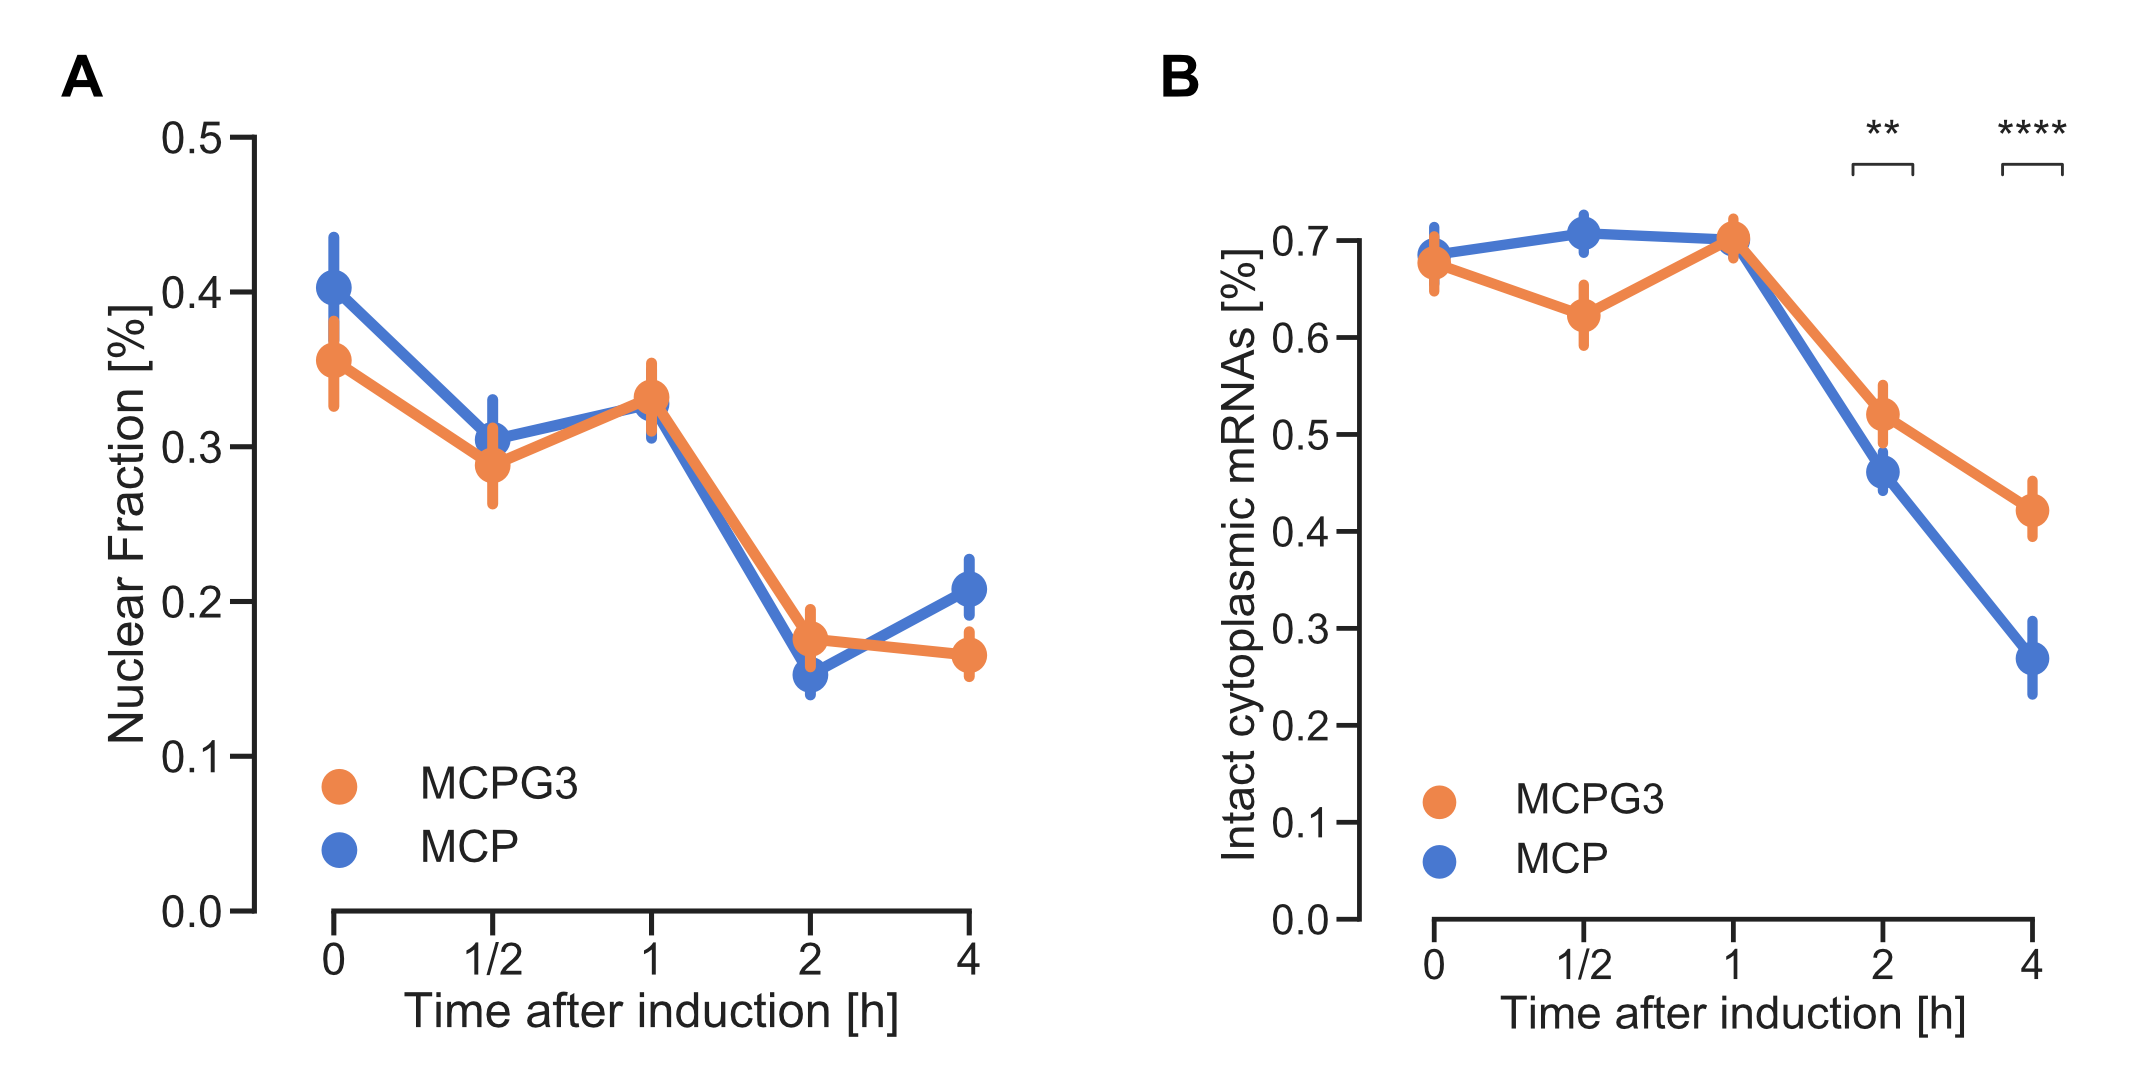
\includegraphics[width=\linewidth]{images/figure5}
    \caption{\textbf{mRNA stability increases by G3BP1 tethering.}
        (A) The fraction of nuclear mRNAs (of total cellular mRNAs)
            at different time points after induction.
        (B) Percentage of intact cytoplasmic mRNAs at different time points.
        (A and B) Number of cells quantified (ascending, MCP then MCPG3):
            117, 154, 200, 175, 55, 114, 148, 167, 111, 132. Single replicate.
    }
    \label{fig:mcp_treat}
\end{figure}


\section{How can the SunTag reporter be improved?} \label{spaghetti}

The original design of the SunTag cassette consists of 24 GCN4 repeats.
These completely disordered repeats have previously lead to the observations of decreased \textit{Renilla} luciferase activity and lower induction rates than \textit{Renilla} luciferase without SunTag.
In an attempt to improve the SunTag based translation imaging system, a spaghetti monster reporter was made.
Spaghetti monster green fluorescent proteins (smGFP) are essentially a non-fluorescent green fluorescent protein's (GFP) beta-barrel used to attach small epitope tags \cite{viswanathan_high-performance_2015}.
Here, three GCN4 repeats each were placed at the N-terminus, C-terminus, and 10/11-loop of the GFP beta-barrel as shown in Figure \ref{fig:spaghetti}A.
Previously, other tags, such as influenza hemagglutinin (HA), were used and visualized with frankenbodies (single-chain antibodies targeting various tags) \cite{zhao_genetically_2019}.
In this study, I attempt to combine SunTag imaging with smGFP constructs.

Initially, while testing the reporter functionality the new reporter showed an approximative 4-fold increase in luciferase activity compared to the standard SunTag reporter (Figure \ref{fig:spaghetti}B).
A \textit{Renilla} reporter was used as control which does not contain any GCN4 repeats.
While the smGFP reporter drastically increases activity, it does not yet reach the levels of the control.
It must be noted, that the control construct does not contain an FKBP tag which has lowered the luciferase activity in previous experiments by enhancing the degradation of the tagged protein \cite{bonger_small_2011}.

To test whether this new reporter allows the visualization of translation sites in live cells, stable cell lines were created and observed after 1 hour of induction.
From a representative image in Figure \ref{fig:spaghetti}C, one can see that cells typically have more, slightly dimmer translation sites.
Quantification of images showed a significant increase in the number of translation sites per cell compared to the cells expressing the standard SunTag reporter (Figure \ref{fig:spaghetti}D).
The brightness of individual spots decreased around 2.7 fold (Figure \ref{fig:spaghetti}E).
This decrease can be explained by a lower number of GCN4 repeats available for the scFv to bind.
Whereas the standard SunTag has 24 GCN4 repeats, smGFP only has 9 leading to a binding site difference of 2.6$\overline{\mbox{6}}$ to 1.
This suggests that the scFv binds to both tags with full occupancy.

Taken together, this study proposes a new SunTag reporter which increases translational activity by greatly increasing the number of active translation sites.
This new reporter allows for shorter induction times with higher mRNA numbers.

\begin{figure}[h]
    \centering
    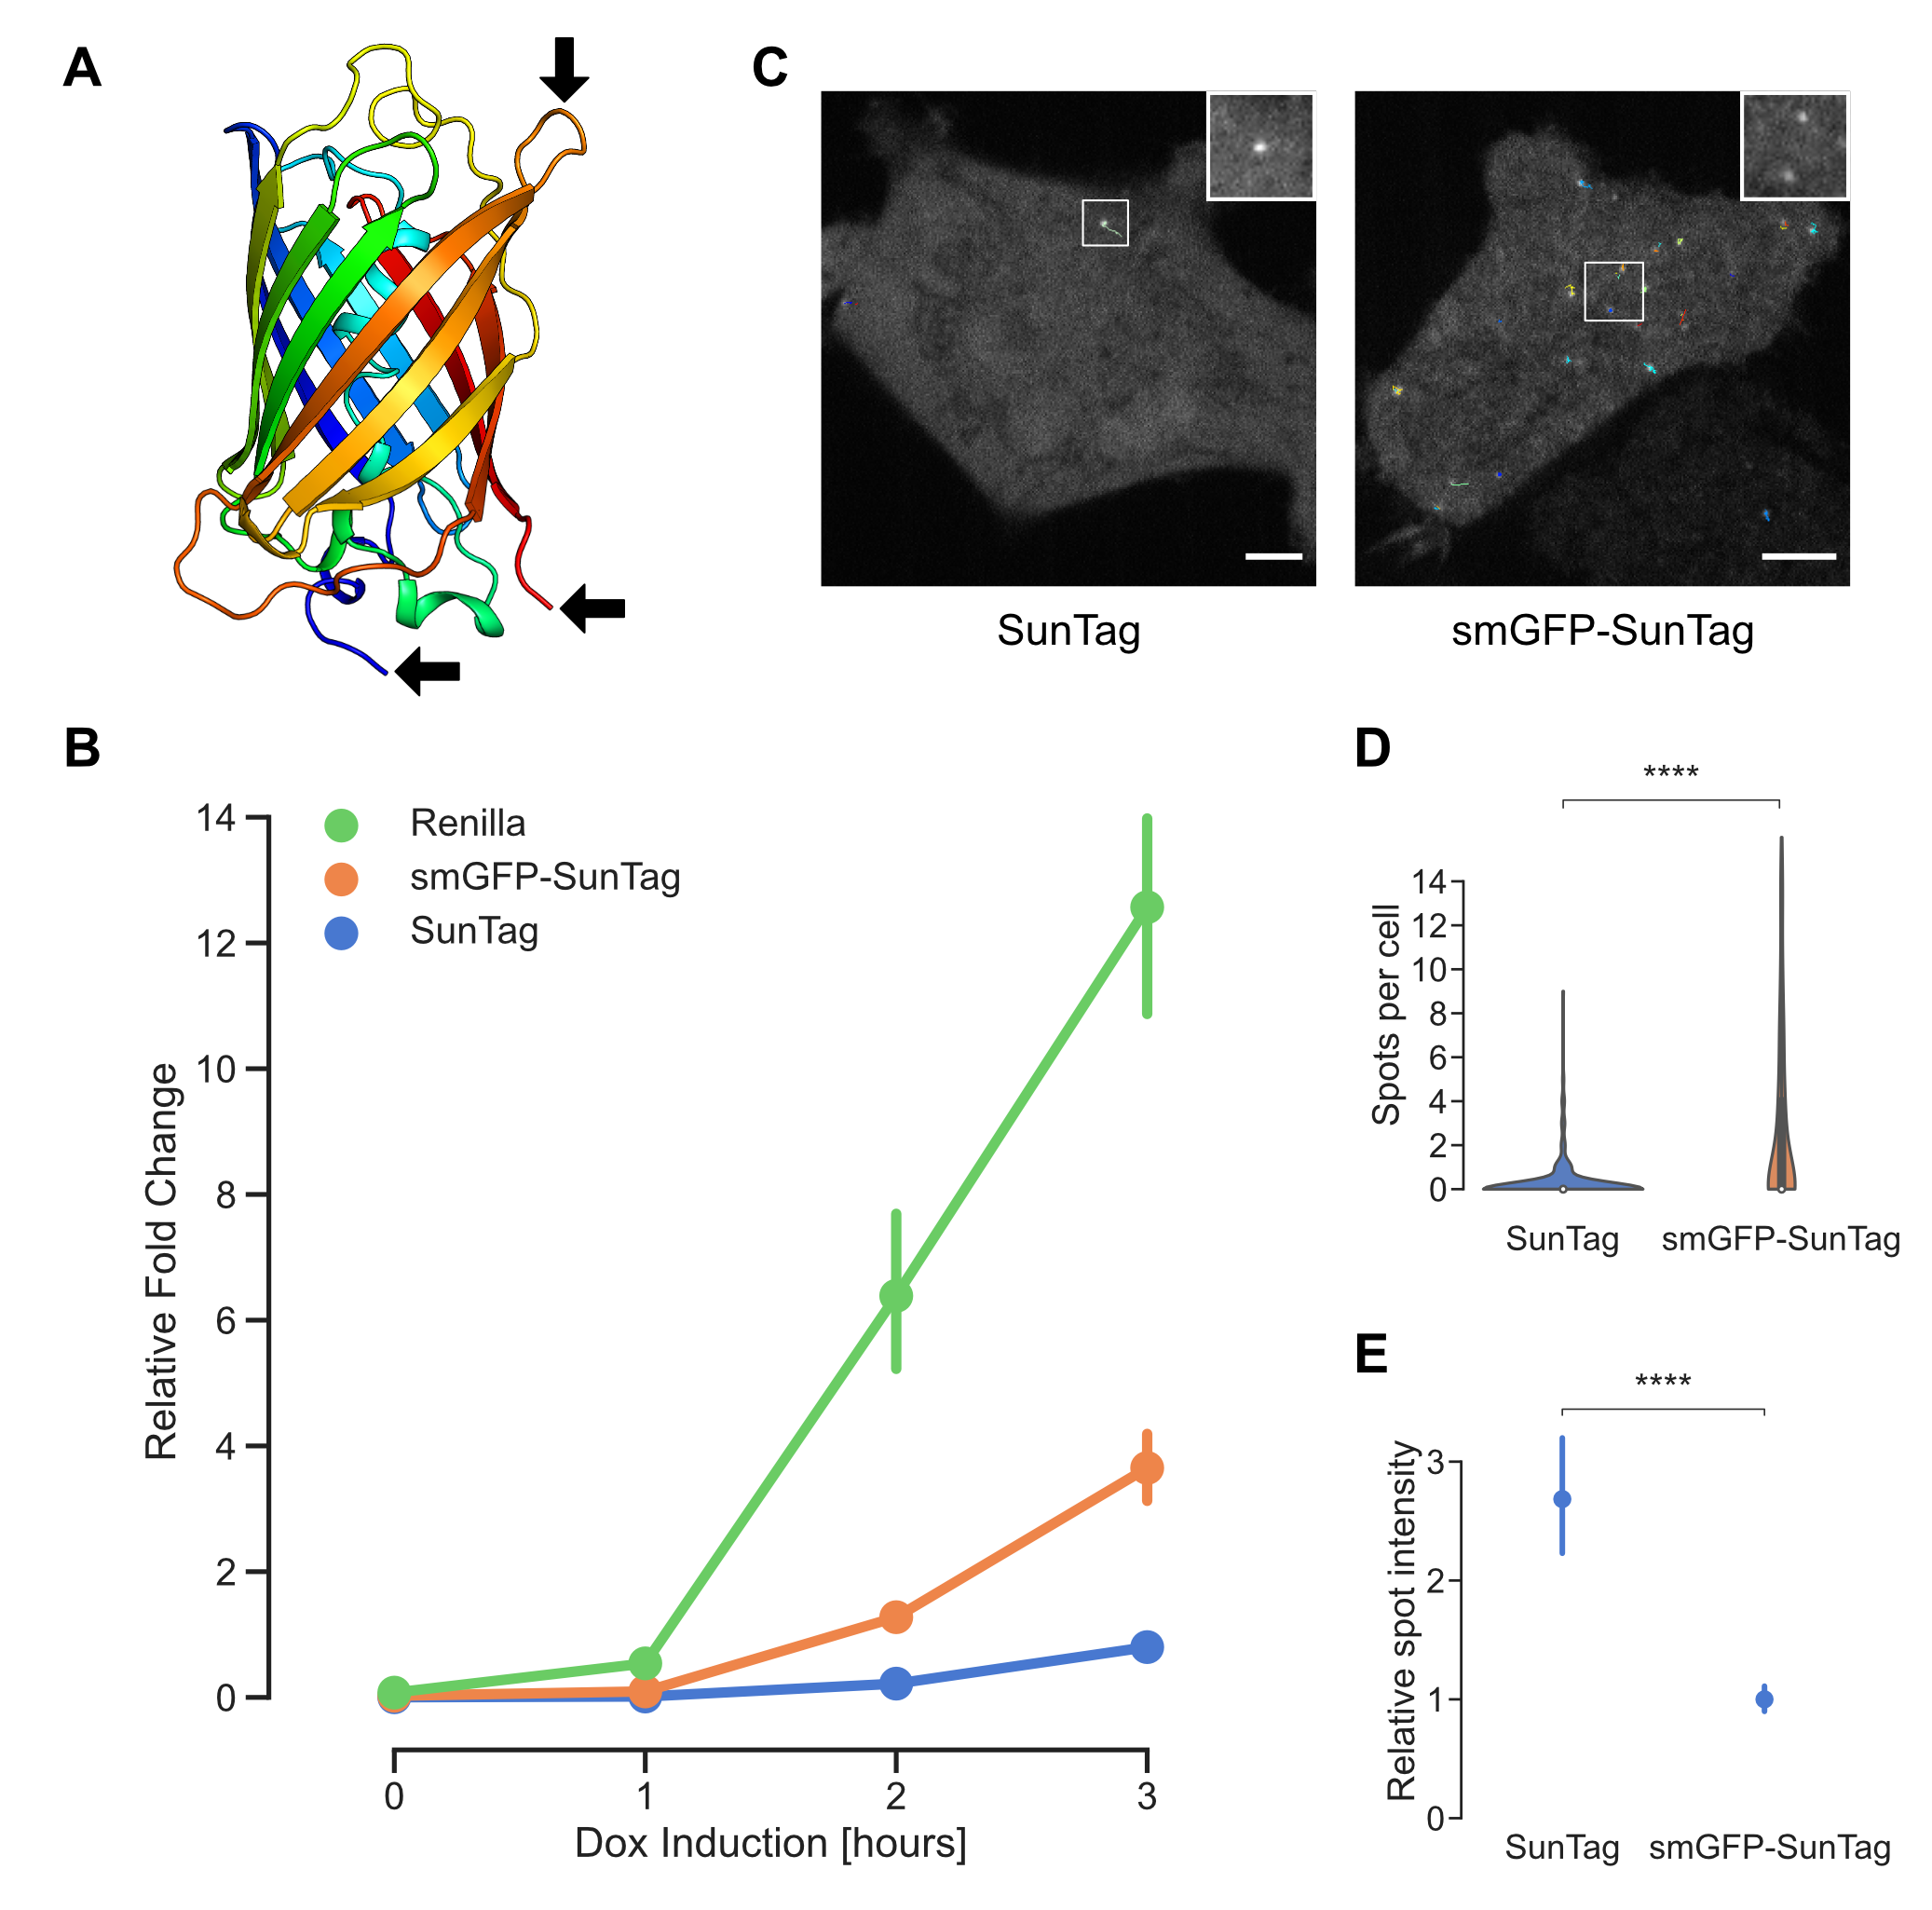
\includegraphics[width=\linewidth]{images/figure6}
    \caption{\textbf{smGFP SunTag reporter increases transcript numbers.}
        (A) Structural overview of GCN4 repeat placement on the smGFP beta-barrel (PDB ID: 1GFL \cite{yang_molecular_1996}).
        (B) Relative luciferase activity comparing the standard SunTag reporter,
            the smGFP SunTag reporter (smGFP-SunTag), and a \textit{Renilla} reporter without SunTag cassette.
        (C) Representative fluorescence images. Each recorded mRNA track is 
            visualized with a unique color. Scale bar, 10 \textmu m.
            The inset shows spots from raw images without brightness corrections.
        (D) Quantification of translation site count per cell.
            The number of cells quantified (left to right): 286, 233.
        (E) Average spot intensity normalized to the smGFP reporter.
            The number of spots quantified (left to right): 36, 39. Two replicates.
        (C, D, and E) Live imaging experiment with stable cell lines imaged after 1 hour
            of induction.
    }
    \label{fig:spaghetti}
\end{figure}